\documentclass{article}
\usepackage{graphicx,fancyhdr,amsmath,amssymb,amsthm,subfig,url,hyperref}
\usepackage[margin=1in]{geometry}
\usepackage[brazilian]{babel}
\usepackage[utf8]{inputenc}
\usepackage{mathtools}
\usepackage{amssymb}
\usepackage{graphics}
\usepackage{fancyhdr}
\usepackage{lastpage}

%----------------------- Macros and Definitions --------------------------

%%% FILL THIS OUT
\newcommand{\studentname}{Bruno H. L. N. Peixoto}
\newcommand{\uspid}{7206666}
\newcommand{\uspmail}{bruno.peixoto@usp.br}
\newcommand{\esnumber}{1}
%%% END

\renewcommand{\theenumi}{\bf \Alph{enumi}}

\fancypagestyle{plain}{}
\pagestyle{fancy}
\fancyhf{}
\fancyhead[RO,LE]{\sffamily\bfseries\large Universidade de São Paulo}
\fancyhead[LO,RE]{\sffamily\bfseries\large PTC5611 Controle Digital de Sistemas Dinâmicos}
\cfoot{Página \thepage \hspace{1pt} de \pageref{LastPage}}	
\renewcommand{\headrulewidth}{1pt}

\graphicspath{{figures/}}

%-------------------------------- Title ----------------------------------

\title{Lista de exercícios \esnumber}
\author{\studentname \qquad Número USP: \uspid \qquad E-mail USP: \uspmail}

%--------------------------------- Text ----------------------------------

\begin{document}
\maketitle

\section*{Exercício 1}
\begin{enumerate}
\item %A

Por hipótese, a frequência de amostragem utilizada satisfaz o critério de Nyquist \footnote{$\omega_s \geq 2\omega_0$}. Como $t = kT_s = \frac{k}{f_s}$:

\begin{equation}
\label{eq:ex1a}
x[k] = cos(k \frac{\omega}{f_s})  \stackrel{!}{=} cos(k \alpha) \Longleftrightarrow \alpha = \frac{\omega}{f_s}
\end{equation}

\begin{equation}
\therefore \omega = 250\pi \frac{rad}{s}
\end{equation}

\begin{figure}[!h]
	\center
	\includegraphics[width=0.7\textwidth]{./images/ex1a.eps}
	\caption{Curva original e série amostrada}
	\label{fig:boat1}
\end{figure}

\item %B
Por (\ref{eq:ex1a}), conclui-se que $f_s = 12$ $kHz$. Dada frequência do sistema de $4000\pi \frac{rad}{s}$, pelo teorema de Nyquist $\omega_s \stackrel{!}{>} 8000\pi \frac{rad}{s} \approx 24000 \frac{rad}{s}$. Devido à violação, não é possível reconstruir o sinal por meio de um passa-baixas ideal. 

\item %C
Para sinais senoidais amostrados com frequência $f_s$, tem-se que, para uma mesma série $x[n] = cos(\alpha n)$, os possíveis sinais advindos deste são $x(t) = cos(2 \pi (f_0 + f_s)t) \mbox{, } k \in \mathbb{N} \mbox{, } \omega = 2 \pi f$. Por \ref{eq:ex1a}, tem-se que $\omega_0 = \frac{5\pi}{4} \frac{rad}{s}$. Assim, dois possíveis sinais para a série fornecida são $x_1(t) = cos(\frac{5\pi}{4} t )$ e $x_2(t) = cos(\frac{85\pi}{4} t)$.

\end{enumerate}

\section*{Exercício 2}

\begin{enumerate}
\item %A

As demonstrações estão enunciadas abaixo:

\begin{itemize}
	\item $Z\{\sum_{i=0}^{n}x[i] \} = \frac{1}{1-z^{-1}}X(z)$
	
	\begin{equation}
	\begin{split}
	Z\{\sum_{i=0}^{n}x[i] \} & = \sum_{n=0}^{\infty} z^{-n} \sum_{i=0}^{n} x[i] \\
	& = x[0] + z^{-1} \sum_{i=0}^{1} x[i] + z^{-2} \sum_{i=0}^{2} x[i] + \cdots \\
	& = x[0] \sum_{i=0}^{\infty} z^{-i} + x[1] \sum_{i=1}^{\infty} z^{-i} + \cdots + x[k] 
	\underbrace{\sum_{i=k}^{\infty} z^{-i}}_{\frac{z^{-k}}{1 - z^{-1}}} + \cdots\\
	& = x[0] \frac{1}{1 - z^{-1}} + x[1] \frac{z^{-1}}{1 - z^{-1}} + \cdots \\
	& = \frac{1}{1 - z^{-1}} \underbrace{\sum_{i=0}^{\infty} x[i].z^{-i}}_{\coloneqq X(z)}
	\end{split}
	\end{equation}

	\begin{equation}
	\therefore Z\{\sum_{i=0}^{n}x[i] \} = \frac{1}{1-z^{-1}}.X(z) \hspace{10pt} \blacksquare
	\end{equation}
	
	\item $Z\{\sum_{i=0}^{n}x[i-1] \} = \frac{z^{-1}}{1-z^{-1}}X(z)$

	\begin{equation}
	\begin{split}
	Z\{\sum_{i=0}^{n}x[i] \} & = \sum_{n=0}^{\infty} z^{-n} \sum_{i=0}^{n} x[i-1] \\
	& = x[-1] + z^{-1} \sum_{i=0}^{1} x[i-1] + z^{-2} \sum_{i=0}^{2} x[i-1] + \cdots \\
	& = \underbrace{x[-1]}_{\coloneqq 0} \sum_{i=0}^{\infty} z^{-i} + x[0] \sum_{i=1}^{\infty} z^{-i} + \cdots \\
	& = x[0] \frac{z^{-1}}{1 - z^{-1}} + x[1] \frac{z^{-2}}{1 - z^{-1}} + \cdots \\
	& = \frac{z^{-1}}{1 - z^{-1}} \underbrace{\sum_{i=0}^{\infty} x[i].z^{-i}}_{\coloneqq X(z)}
	\end{split}
	\end{equation}

	\begin{equation}
	\therefore Z\{\sum_{i=0}^{n}x[i-1] \} = \frac{z^{-1}}{1-z^{-1}}.X(z) \hspace{10pt} \blacksquare
	\end{equation}

	\item $\lim\limits_{z \rightarrow 1} X(z) = \sum_{i=0}^{\infty}x[i]$

	\begin{equation}
	\lim\limits_{z \rightarrow 1} X(z) & = \lim\limits_{z \rightarrow 1} \sum_{i=0}^{\infty} x[i].z^{-i} = \sum_{i=0}^{\infty} x[i]
	\end{equation}
	
	\begin{equation}
	\begin{split}
	\therefore \lim\limits_{z \rightarrow 1} X(z) = \sum_{i=0}^{\infty}x[i] \hspace{10pt} \blacksquare
	\end{split}
	\end{equation}
	
\end{itemize}

\item\label{item:ex2b} %B
Dada função $x_1(t) = \frac{1}{a} \left( 1 - e^{-at} \right)$, por definição tem-se que:

	\begin{equation}
	\begin{split}
	Z\{x_1(t)\} = X_1(z) & = \sum_{i=0}^{\infty} x_1(i Ts).z^{-i} \\
	& = \frac{1}{a} \sum_{i=0}^{\infty} \left( 1 - e^{-a T_s i} \right)z^{-i} \\
	& = \frac{1}{a} \sum_{i=0}^{\infty} z^{-i} - \frac{1}{a} \sum_{i=0}^{\infty} \underbrace{e^{-a T_s i}.z^{-i}}_{(z.e^{aT_s})^{-i}}
	\end{split}
	\end{equation}
	
Se $|z| > 1 \wedge |z| > e^{aT_s}$, então:
	
	\begin{equation}
	\begin{split}
	\frac{1}{a} \sum_{i=0}^{\infty} z^{-i} - \frac{1}{a} \sum_{i=0}^{\infty} e^{-a T_s i}.z^{-i} & = \frac{1}{a} (\frac{1}{1-z^ {-1}} - \frac{1}{1-e^{-aT_s} z^ {-1}}) \\
	& = \frac{1}{a} \frac{(1 - e^{-aT_s})z^{-1}}{(1-z^{-1})(1-e^{-aT_s} z^ {-1})}
	\end{split}
	\end{equation}
	
Portanto
	
	\begin{equation}
	X_1(z) = \frac{1}{a}  \frac{(1 - e^{-aT_s})z^{-1}}{(1-z^{-1})(1-e^{-aT_s} z^ {-1})}
	\end{equation}

De mesma forma, dada função $x_2(t) = $t^2 e^{-a t}$, por definição tem-se que:

	\begin{equation}
	\begin{split}
	Z\{x_2(t)\} = X_2(z) & = \sum_{i=0}^{\infty} x_2(i Ts).z^{-i} \\
	& = \sum_{i=0}^{\infty} \left( i^2 T_s^2 e^{-a T_s i} z^{-i} \right) \\
	& = \sum_{i=0}^{\infty} T_s^2 i^2 e^{-a T_s i} z^{-i}
	\end{split}
	\end{equation}
	
Por meio da propriedade da transformada $\mathcal{Z}\{n X[n]\} \coloneqq -z \frac{d}{dz} X(z)$, segue

    \begin{equation}
    x[n] = e^{-an} & \rightarrow -z \frac{d}{dz} \mathcal{Z}\{e^{-an}\} = \mathcal{Z}\{n e^{-an}\} \mbox{, } n = T_s i \mbox{, } i \in \mathbb{N}
    \end{equation}
    
e

    \begin{equation}
    x[n] = n e^{-an} & \rightarrow -z \frac{d}{dz} \mathcal{Z}\{n e^{-an}\}} = \mathcal{Z}\{n^2 e^{-an}\} \mbox{, } n = T_s \mbox{, } i \in \mathbb{N}
    \end{equation}

Logo

    \begin{equation}
    \begin{split}
    \mathcal{Z}\{e^{-an}\} & = \frac{1}{1 - e^{-a T_s} z^{-1}} \Rightarrow \\
    \frac{d}{dz} \mathcal{Z}\{e^{-an}\} & = - e^{-a T_s} \frac{z^{-2}}{(1 - e^{-a T_s} z^{-1})^2} \\
    \mathcal{Z}\{n e^{-an}\} \coloneqq -z \frac{d}{dz} \mathcal{Z}\{e^{-an}\} & = e^{-a T_s} \frac{z^{-1}}{(1 - e^{-a T_s} z^{-1})^2}
    \end{split}
    \end{equation}

e

    \begin{equation}
    \begin{split}
    \mathcal{Z}\{n e^{-an}\} & = e^{-a T_s} \frac{z^{-1}}{(1 - e^{-a T_s} z^{-1})^2} \Rightarrow \\ \frac{d}{dz} \mathcal{Z}\{n e^{-an}\} & = e^{- a T_s} \frac{z^{-2}(1 - e^{-a T_s} z^-1)^2 - 2(1 - e^{-a T_s} z^{-1}) e^{-a T_s} z^{-2}}{(1 - e^{-a T_s} z^{-1})^3} \\ 
    & = - e^{-a T_s} \frac{z^{-2} (1 + e^{-a T_s} z^{-1})}{(1 - e^{- a T_s} z^-1)^3} \\
    \mathcal{Z}\{n^2 e^{-a n}\} \coloneqq -z \frac{d}{dz} \mathcal{Z}\{n e^{-a n}\} & = e^{-a T_s} \left( \frac{z^{-1}(1 + e^{-a T_s} z^{-1})}{(1 - e^{-a T_s} z^{-1})} \right)
    \end{split}
    \end{equation}

Portanto 

\begin{equation}
\mathcal{Z}\{n^2 e^{-a n}\} = e^{-a T_s} \frac{z^{-1}(1 + e^{-a T_s} z^{-1})}{(1 - e^{-a T_s} z^{-1})}
\end{equation}

\item %C
A equação das diferenças pode ser colocada da seguinte forma:

\begin{equation}
\sum_{i=0}^{m} b_i y[n-i] = \sum_{i=0}^{n} a_i x[n-i]
\end{equation}

com parâmetros dados por $m = n = 3$ e $a_i, b_i$, $i = 1, 2, 3$ dados por $a_0 = 1$, $a_1 = -0.9737$, $a_2 = 0.8101$, $a_3 = 0.8151$, $a_1 = -0.0515$, $b_0 = 0.4108$, $b_1 = -1.0094$, $b_2 = 1.0094$ e $b_3 = 0.4108$ .

Após aplicar a transformada Z no sistema, temos que

\begin{equation}
G(z) = \frac{Y(Z)}{X(z)} = \frac{\sum_{i=0}^{m} b_{i} z^{-i}}{\sum_{i=0}^{n} a_{i} z^{-i}} = \frac{\sum_{i=0}^{m} b_{m-i} z^{i}}{\sum_{i=0}^{n} a_{n-i} z^{i}}
\end{equation}

Assim, as raízes do numerador e denominador, nomeadamente zeros e pólos, são respectivamente $z = \{1.38 \pm 1.18 i, -0.3\}$ e $p = \{0.45 \pm 0.74i, 0.068\}$.

\end{enumerate}

\section*{Exercício 3}
Dado sinal discreto $a[n]$ resultado da primeira soma à esquerda no diagrama de blocos, temos que:

\begin{equation}
\begin{split}
\label{eq:ex31}
A(z) = 2 X(z) - 2 z^{-1} X(z) 0.3 - 0.5 z^{-2} Y(z)
\end{split}
\end{equation}

De mesma forma,

\begin{equation}
\label{eq:ex32}
Y(z) = -z^2 X(z) + A(z) - z^{-1} Y(z)
\end{equation}

Substituindo-se (\ref{eq:ex31}) em (\ref{eq:ex32}), obtém-se:

\begin{equation}
\begin{split}
-z^{-2} X(z) + 2 X(z) - 0.6  z^{-1} X(z) - 0.5 z^{-2} Y(z) - z^{-1} Y(z) \\
\frac{Y(z)}{X(z)} = \frac{- z^{-2} - 0.6 z^{-1} + 2}{0.5 z^-2 + z^{-1} + 1} = \frac{2 z^{2} - 0.6 z - 1}{z^2 + z + 0.5}
\end{split}
\end{equation}

Os pólos do sistema é estável pois seus pólos $z = \pm\frac{\sqrt{2}}{2}$ encontram-se no interior do circulo unitário, região estável em tempo discreto.

A imagem (\ref{fig:ex3sim}) refe-se à simulação do diagrama fornecido e a função de transferência encontrada. Perceba que ambos se sobrepõe nos instantes múltiplos do tempo de amostragem.

\begin{figure}[!h]
	\center
	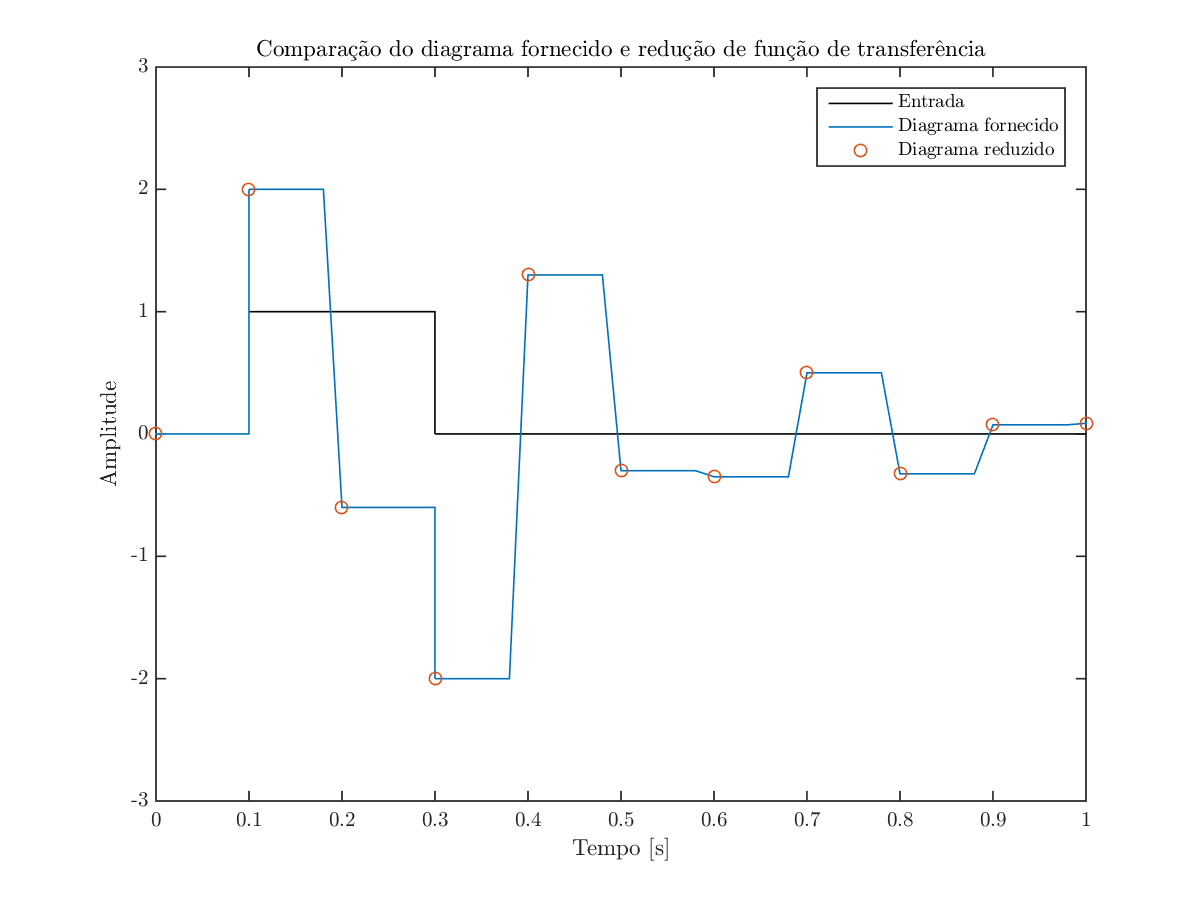
\includegraphics[width=\textwidth]{./images/ex31.png}
	\caption{Entrada do sistema amostrado e saídas do diagrama amostrado e função de transferência equivalente}
	\label{fig:ex3sim}
\end{figure}

\begin{figure}[!h]
	\center
	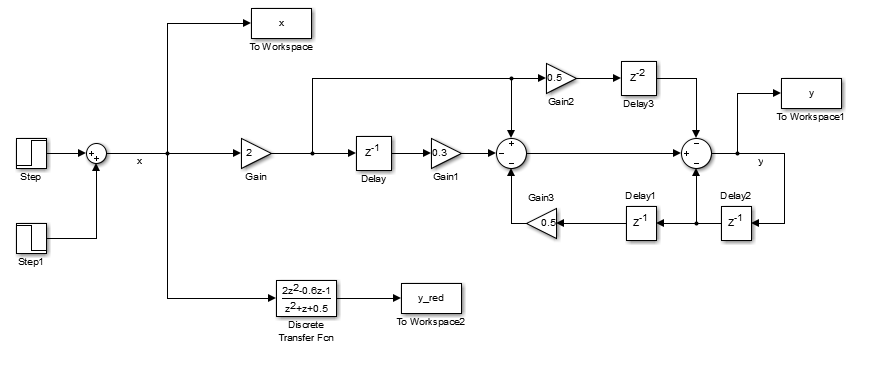
\includegraphics[width=\textwidth]{./images/ex3simulink.tif}
	\caption{Entrada do sistema amostrado e saídas do diagrama amostrado e função de transferência equivalente}
	\label{fig:ex3diag}
\end{figure}

\section*{Exercício 4}

A conversão sem aproximação do espaço contínuo para discreto com mantenedor de ordem zero (ZOH) satisfaz a seguinte equação:

\begin{equation}
G(z) \coloneqq (1-z^{-1}) \mathcal{Z}\left\{\mathcal{L}^{-1}\left\{\frac{G(s)}{s}\right\}\right\}
\end{equation}

Desta forma

\begin{equation}
\label{eq:ex41}
\frac{G(s)}{s} = H(s) = \frac{K}{s(s+a)}
\end{equation}

Pelo método de expansão de frações parciais, a equação (\ref{eq:ex41}) apresenta a seguinte forma

\begin{equation}
H(s) = \frac{A}{s} + \frac{B}{(s+a)} 
\end{equation}

Onde 

\begin{equation}
A = H(s) s \bigg\rvert_{s=0} = \frac{K}{a} \mbox{ e } B = H(s) (s+a)\bigg\rvert_{s=-a} = -\frac{K}{a}
\end{equation}

Logo

\begin{equation}
H(s) = \frac{K}{a} \left( \frac{1}{s} - \frac{1}{s+a} \right)
\end{equation}

A função de transferência acima exceto ao fator de escala $j$ foi obtida no item (\ref{item:ex2b}). Desta forma

\begin{equation}
\label{eq:lapinv}
\mathcal{L}^{-1}\left\{\frac{G(s)}{s}\right\} = \frac{K}{a}\sigma(t)\left(1+e^{-at}\right)
\end{equation}

Portanto, a função $\mathcal{Z}$ da função (\ref{eq:lapinv}) é dada por

\begin{equation}
G(z) = \frac{K}{a} \frac{(1 - e^{-aT_s}z^{-1})}{(1-z^{-1})(1 - e^{-aT_s}z^{-1})}
\end{equation}

Por fim, por meio da função de transefrência de uma malha fechada \footnote{A equação em malha fechada de um sistema em tempo discreto ou contínuo é dado pela equação $G_{MF}(z) = \frac{G(z)}{1+G(z)}$}, após certa manipulação algébrica é dada por:

\begin{equation}
G_{MF}(z) = K' \frac{z}{z+b}
\end{equation}

onde $K' = \frac{K}{a} (1-e^{-aT_s}) \mbox{ e } b = \left[\left[(1 + \frac{k}{a})\right]e^(-aT_s) - \frac{k}{a} \right] $.

\section*{Exercício 5} Dados: Ts = 0,1 s

\begin{enumerate}
\item % A

\begin{equation}
\begin{split}
s = \frac{z - 1}{T_s} \therefore X(z) = \frac{\frac{z+1}{T_s} + 1}{\frac{z+1}{T_s} + 10} = \frac{z - (1-T_s)}{z - (1-10T_s)} = \frac{z - 0.9}{z} 
\end{split}
\end{equation}

\item % B

\begin{equation}
\begin{split}
s = \frac{z - 1}{T_s z} \therefore X(z) = \frac{\frac{z-1}{T_s z} + 1}{\frac{z-1}{T_s z} + 10} = \frac{(1+T_s) z - 1}{(1 + 10T_s) z + 1} = 0.45 \frac{z - 1.1}{z - 0.5}
\end{split}
\end{equation}

\item % C

\begin{equation}
\begin{split}
s = \frac{2}{T_s} \frac{z - 1}{z+1} \therefore X(z) = \frac{\frac{2}{T_s} \frac{z-1}{z+1} + 1}{\frac{2}{T_s} \frac{z-1}{z+1} + 10} = \frac{(2+T_s)z + (T_s - 2)}{(2 + 10T_s) z + (10 T_s - 2)} = \frac{2.1z - 1.9}{3z - 1} = 0.7\frac{z-0.63}{z-0.33}
\end{split}
\end{equation}

\item % D
Dados: $\omega_c = 3 \frac{rad}{s}$

\begin{equation}
s = \frac{\omega_c}{\tan{\frac{\omega_c T_s}{2}}} \frac{z-1}{z+1} \therefore X(z) = \frac{\frac{\omega_c}{\tan(\frac{\omega_c T_s}{2})} \frac{z-1}{z+1} + 1}{\frac{\omega_c}{\tan(\frac{\omega_c T_s}{2})} \frac{z-1}{z+1} + 10} = \frac{(\tan{\frac{\omega_c T_s}{2}} + \omega_c) z + (\tan{\frac{\omega_c T_s}{2}} - \omega_c)}{(10 \tan{\frac{\omega_c T_s}{2}} + \omega_c) z + (10 \tan{\frac{\omega_c T_s}{2}} - \omega_c)} 
\end{equation}

Como $\frac{\omega_c T_s}{2} \ll 1$ e $\tan{\theta} \approx \theta$, então $\tan{\frac{\omega_c T_s}{2}} \approx \frac{\omega_c T_s}{2}$. Assim

\begin{equation}
X(z) = \frac{3.15\ - 2.85}{4.15z - 1.5} = 0.76 \frac{z - 0.9}{z - 0.36}
\end{equation}

\item % E
Todo pólo e zero da planta pode ser mapeado diretamente para o espaço $\mathcal{Z}$ pela relação $z = e^{s T_s}$. O ganho da função em regime estacionário devem ambos em espaço discreto quanto contínuo iguais.

\begin{equation}
\lim\limits_{z \rightarrow 1} (1 - z^{-1})X(z) \stackrel{!}{=} \lim\limits_{s \rightarrow 0} s X(s) 
\end{equation} 

Desta forma.

\begin{equation*}
\begin{split}
K_z \frac{1 - e^{-Ts}}{1 - e^{-10Ts}} = \frac{1}{10} \Rightarrow K_z = 10 \frac{1 - e^{-10T_s}}{1 - e^{-T_s}} \approx 1.59
\end{split}
\end{equation*}

Portanto

\begin{equation}
X(z) = 1.59 \frac{z - 0.9}{z - 0.37}
\end{equation}

\end{enumerate}

\section*{Exercício 6}
Para que a função de transferência em malha fechada do sistema seja de segunda ordem, o controlador deve ser proporcional.O polinômio característico da função de transferência é:

\begin{equation}
P(s) = s^2 + 7s + k \stackrel{!}{=} s^2 + 2 \zeta \omega_n + \omega_n^2
\end{equation}

O tempo de subida é dada pela identidade:

\begin{equation}
\label{eq:sobressinal}
t^{0\% - 100\%}_{r}(\omega_n, \zeta) = \frac{\pi - \theta(\zeta)}{\omega_d(\omega_n, \zeta)} \mbox{, com } \theta(\zeta) = \tan^{-1}\frac{\sqrt{1 - \zeta^2}}{\zeta} \mbox{ e } \omega_d(\omega_n, \zeta) = \omega_n \sqrt{1-\zeta^2}
\end{equation}

De mesma forma, o sobressinal é dado por:

\begin{equation}
\label{eq:sobressinal}
M(\zeta) = e^{-\pi \frac{\zeta}{\sqrt{1-\zeta^2}}}
\end{equation}

Caso (\ref{eq:sobressinal}) for bijetora, $\exists g(M) = \zeta \mbox{, } g: \zeta \rightarrow g(zeta) \mbox{, } M \circ g = M$. De fato $g(M) = \sqrt{\frac{\log^2{M}}{\pi^2 - \log^2{M}}}$. Assim, $\zeta \approx 0.672$

Para $\zeta$ fixo, analogamente, $\exists h(t_r) = \zeta\mbox{, }h: t_r \rightarrow h(zeta)\mbox{, } t_r(\zeta) \circ h = t_r$. De fato, $g(t_r) = \frac{\pi - \theta}{\omega_d(\zeta, t_r)}$. Assim, para $\zeta = 0.672$, então $\omega_n = 4.46$.  Como $\omega_n^2 = k$, então $k = 19.96$.

\section*{Exercício 7}

Função de transferência de controlador PID:

\begin{equation}
C(s) = K_p\left(1 + \frac{1}{T_i s} + T_d s\right)
\end{equation}

\begin{enumerate}
	\item % A
	Seja a aproximação retangular para trás dada por $s = \frac{1 - z^{-1}}{2 T_s}$, com auxílio do MATLAB para manipulação simbólica, a função de transferência do controlador PID é dada por:
	
	\begin{equation}
	C(z) = K_p \frac{b_2 z^{-2} + b_1 z^{-1} + b_0}{a_2 z^{-2} + a_1 z^{-1} + a_0}
	\end{equation}
	
	com $b_2 = T_i (T_d - T_s) + 4T_s^2$, $b_1 = 2T_i(T_s - T_d)$, $b_0 = T_i T_d$, $a_2 = -2T_i T_s$, $a_1 = 2 T_i T_s$ e $a_0 = 0$.

	SIMULAÇÃO!

	\item % B
	SIMULAÇÃO!
	
	\item %C
	SIMULAÇÃO!
	
\end{enumerate}

\section*{Exercício 7}

\section*{Exercício 8}

\section*{Exercício 9}

\section*{\Huge Apêndice}

\end{document}
